\section{Pakete deinstallieren}In diesem Dialog k�nnen Sie Pakete von einem Client entfernen.\\
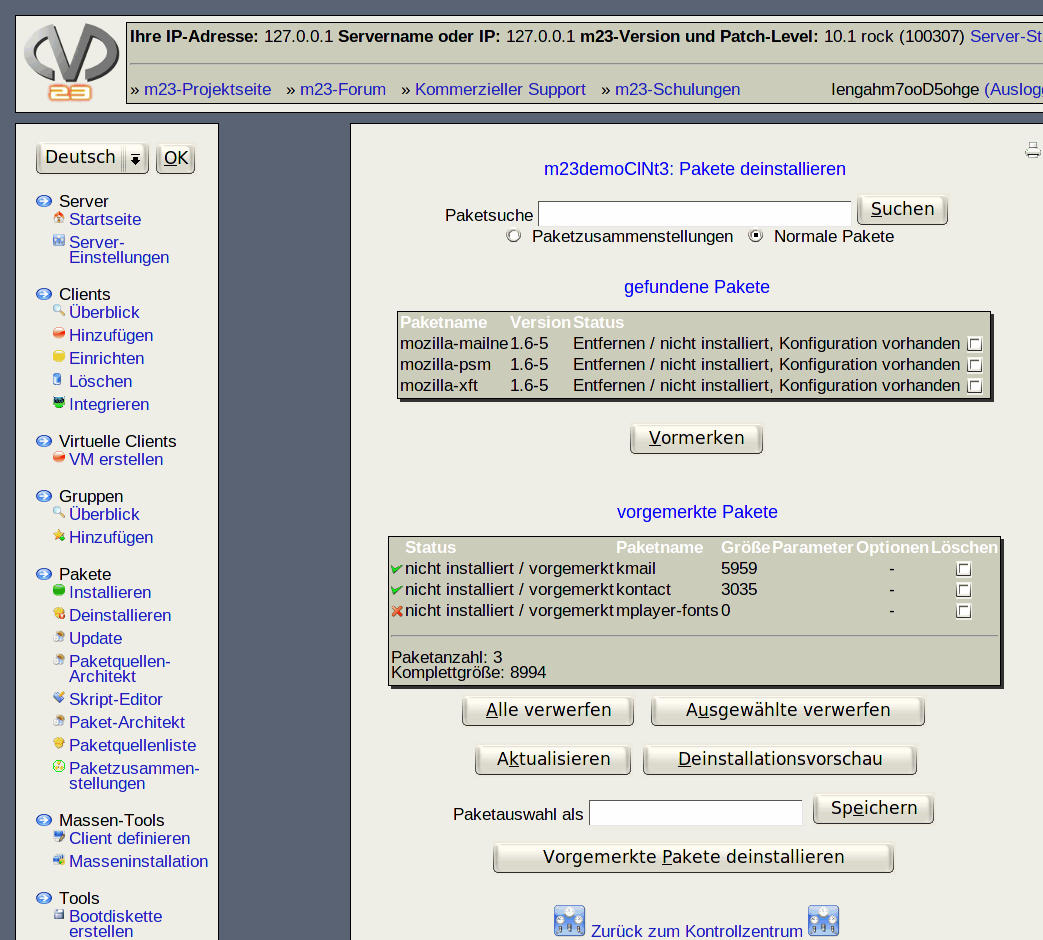
\includegraphics[scale=0.4]{/mdk/doc/manual/screenshots/de/deinstall_packages.png} \\
\subsection{Hinweis}
m23 unterscheidet drei verschiedene Paketarten:\\
\begin{itemize}
\item \textbf{Paketzusammenstellungen:} Sind eine Zusammenstellung von verschiedenen Paketen. Sie k�nnen aus einer Vielzahl von Anwendungen ein Paket schn�ren und so die Installation von identischen Programmpaketen auf verschiedenen Rechnern enorm erleichtern.\\
\item \textbf{Normale Pakete:} Sind normale Programmpakete. Dies sind in der Regel einzelne Programme.\\
\item \textbf{Spezialpakete (f�r erfahrene Benutzer):} Enthalten Pakete, die Spezialaufgaben wie Formatieren etc. durchf�hren. Spezialpakete sollten nur durch erfahrene Benutzer angewendet werden.\\
\end{itemize}
\subsection{Deinstallation von Paketen}
\begin{enumerate}
\item  W�hlen Sie \textit{"Paketzusammenstellungen"} oder \textit{"Normale Pakete"} aus.\\
\item  Geben Sie bei \textit{"Paketsuche"} den Suchbegriff f�r das gew�nschte Paket ein. Lassen Sie das Suchfeld leer, wenn Sie alle Pakete des Clients sehen m�chten.\\
\item  Unter \textit{"gefundene Pakete"} finden Sie alle Pakete, die Ihren Suchparametern entsprechen.\\
\item  Klicken Sie bei den gew�nschten Paketen die Checkbox an.\\
\item  Merken Sie die gew�hlten Pakete durch Klick auf \textit{"Vormerken"} vor.\\
\item  Wiederholen Sie bei Bedarf Schritt 1-5.\\
\end{enumerate}
Nun haben Sie Pakete f�r die Deinstallation vorgemerkt.  Ein gr�ner Haken gibt an, da� dieses Paket zu installieren ist und ein rotes Kreuz, da� dieses Paket vom Client entfernt werden soll. Sie k�nnen die Liste dieser Pakete durch einen Klick auf den Button \textit{"Alle verwerfen"} l�schen oder Pakete ausw�hlen und diese durch \textit{"Ausgew�hlte verwerfen"} entfernen.\\
Schlie�en Sie Ihre Auswahl durch Klick auf \textit{"Vorgemerkte Pakete deinstallieren"} ab.\\
\subsection{Deinstallationsvorschau}
Vor der wirklichen Deinstallation k�nnen Sie �berpr�fen, was die Deinstallation auf dem Client f�r Folgen hat. So k�nnen Sie vorher sehen, welche zus�tzlichen Pakete entfernt werden. Klicken Sie dazu nach Auswahl der Pakete auf \textit{"Deinstallationsvorschau"}. Nach einem Augenblick sehen Sie ein Protokoll der Deinstallationsvorschau.\\
Eine Deinstallationsvorschau ist allerdings nur dann m�glich, wenn ein einzelner Client und keine Gruppe ausgew�hlt wurde.\\
\subsection{Hinweis zu Paketzusammenstellungen}
Wenn Sie "Paketzusammenstellung" ausw�hlen, k�nnen Sie bestimmen, ob die Pakete auf dem Client installiert oder deinstalliert werden sollen. Au�erdem k�nnen Sie die in der Paketzusammenstellung gespeicherte Aktionen beibehalten. Dies erlaubt es, Installations- und Deinstallations-Auftr�ge in einer einzigen Zusammenstellung zu benutzen. W�hlen Sie dazu aus der Auswahlliste die gew�nschte Aktion aus.\\
\subsection{Tip}
M�chten Sie Ihre Paketauswahl f�r sp�tere Benutzung sichern, geben Sie nach \textit{"Paketauswahl als"} einen Namen f�r Ihre Zusammenstellung ein und sichern Sie diese mit dem \textit{"Speichern"}-Button. Diese Zusammenstellung steht Ihnen sofort unter \textit{"Paketzusammenstellungen"} zur Verf�gung.\\
